\documentclass[11pt, a4paper, onecolumn]{article}
\usepackage[utf8]{inputenc}
\usepackage{geometry}
\geometry{a4paper, portrait, margin=1in}
\usepackage{graphicx}
\usepackage{tikz}
\usetikzlibrary{arrows}
\usepackage{booktabs} % nice tables
\usepackage[procnames]{listings} % nice code
\usepackage{color}

\title{Natural Computation - Assignment 1}
\author{Stuart Stobie (ss835)}
\date{October 2015}

\begin{document}

\maketitle

\pagebreak

\section{Task 1}

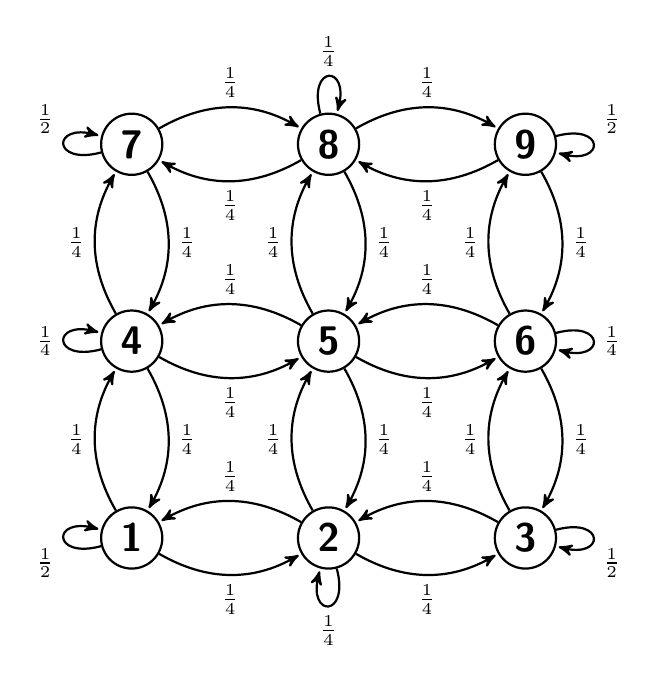
\begin{tikzpicture}[->,>=stealth',shorten >=1pt,auto,node distance=2.5cm,thick,main node/.style={circle,draw,font=\sffamily\Large\bfseries}]

  \node[main node] (1) {1};
  \node[main node] (2) [right of=1] {2};
  \node[main node] (3) [right of=2] {3};
  \node[main node] (4) [above of=1] {4};
  \node[main node] (5) [right of=4] {5};
  \node[main node] (6) [right of=5] {6};
  \node[main node] (7) [above of=4] {7};
  \node[main node] (8) [right of=7] {8};
  \node[main node] (9) [right of=8] {9};

  \path[every node/.style={font=\sffamily\small}]
    (1) edge [bend left] node [left] {\(\frac{1}{4}\)} (4)
        edge [bend right] node [below] {\(\frac{1}{4}\)} (2)
        edge [loop left] node [below left] {\(\frac{1}{2}\)} (1)
    (2) edge [bend left] node [left] {\(\frac{1}{4}\)} (5)
        edge [bend right] node [below] {\(\frac{1}{4}\)} (3)
        edge [bend right] node [above] {\(\frac{1}{4}\)} (1)
        edge [loop below] node [below] {\(\frac{1}{4}\)} (2)
    (3) edge [bend left] node [left] {\(\frac{1}{4}\)} (6)
        edge [bend right] node [above] {\(\frac{1}{4}\)} (2)
        edge [loop right] node [below right] {\(\frac{1}{2}\)} (3)
    (4) edge [bend left] node [left] {\(\frac{1}{4}\)} (7)
        edge [bend right] node [below] {\(\frac{1}{4}\)} (5)
        edge [bend left] node [right] {\(\frac{1}{4}\)} (1)
        edge [loop left] node [left] {\(\frac{1}{4}\)} (4)
    (5) edge [bend left] node [left] {\(\frac{1}{4}\)} (8)
        edge [bend right] node [below] {\(\frac{1}{4}\)} (6)
        edge [bend left] node [right] {\(\frac{1}{4}\)} (2)
        edge [bend right] node [above] {\(\frac{1}{4}\)} (4)
    (6) edge [bend left] node [left] {\(\frac{1}{4}\)} (9)
        edge [loop right] node [right] {\(\frac{1}{4}\)} (6)
        edge [bend left] node [right] {\(\frac{1}{4}\)} (3)
        edge [bend right] node [above] {\(\frac{1}{4}\)} (5)
    (7) edge [loop left] node [above left] {\(\frac{1}{2}\)} (7)
        edge [bend left] node [above] {\(\frac{1}{4}\)} (8)
        edge [bend left] node [right] {\(\frac{1}{4}\)} (4)
    (8) edge [bend left] node [above] {\(\frac{1}{4}\)} (9)
        edge [loop above] node [above] {\(\frac{1}{4}\)} (8)
        edge [bend left] node [right] {\(\frac{1}{4}\)} (5)
        edge [bend left] node [below] {\(\frac{1}{4}\)} (7)
    (9) edge [bend left] node [right] {\(\frac{1}{4}\)} (6)
        edge [loop right] node [above right] {\(\frac{1}{2}\)} (9)
        edge [bend left] node [below] {\(\frac{1}{4}\)} (8);
\end{tikzpicture}

\section{Task 2}

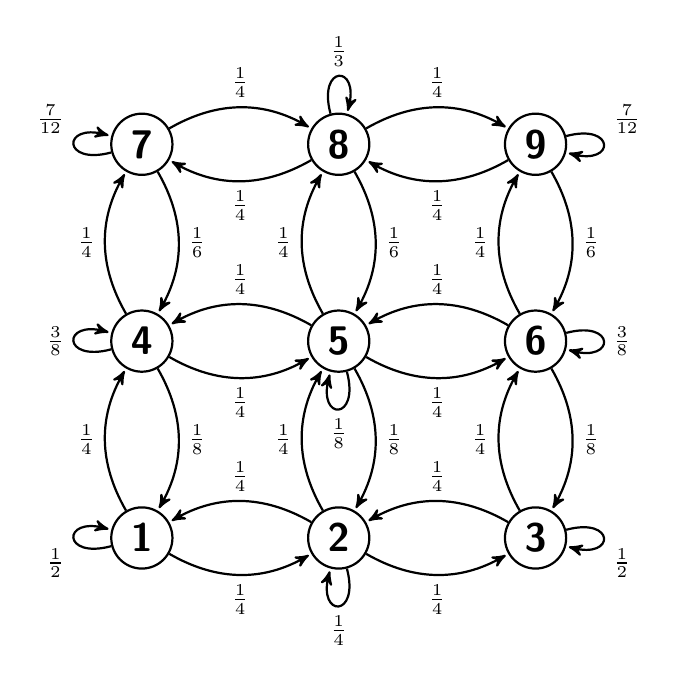
\begin{tikzpicture}[->,>=stealth',shorten >=1pt,auto,node distance=2.5cm,thick,main node/.style={circle,draw,font=\sffamily\Large\bfseries}]

  \node[main node] (1) {1};
  \node[main node] (2) [right of=1] {2};
  \node[main node] (3) [right of=2] {3};
  \node[main node] (4) [above of=1] {4};
  \node[main node] (5) [right of=4] {5};
  \node[main node] (6) [right of=5] {6};
  \node[main node] (7) [above of=4] {7};
  \node[main node] (8) [right of=7] {8};
  \node[main node] (9) [right of=8] {9};

  \path[every node/.style={font=\sffamily\small}]
    (1) edge [bend left] node [left] {\(\frac{1}{4}\)} (4)
        edge [bend right] node [below] {\(\frac{1}{4}\)} (2)
        edge [loop left] node [below left] {\(\frac{1}{2}\)} (1)
    (2) edge [bend left] node [left] {\(\frac{1}{4}\)} (5)
        edge [bend right] node [below] {\(\frac{1}{4}\)} (3)
        edge [bend right] node [above] {\(\frac{1}{4}\)} (1)
        edge [loop below] node [below] {\(\frac{1}{4}\)} (2)
    (3) edge [bend left] node [left] {\(\frac{1}{4}\)} (6)
        edge [bend right] node [above] {\(\frac{1}{4}\)} (2)
        edge [loop right] node [below right] {\(\frac{1}{2}\)} (3)
    (4) edge [bend left] node [left] {\(\frac{1}{4}\)} (7)
        edge [bend right] node [below] {\(\frac{1}{4}\)} (5)
        edge [bend left] node [right] {\(\frac{1}{8}\)} (1)
        edge [loop left] node [left] {\(\frac{3}{8}\)} (4)
    (5) edge [bend left] node [left] {\(\frac{1}{4}\)} (8)
        edge [bend right] node [below] {\(\frac{1}{4}\)} (6)
        edge [bend left] node [right] {\(\frac{1}{8}\)} (2)
        edge [loop below] node [below] {\(\frac{1}{8}\)} (5)
        edge [bend right] node [above] {\(\frac{1}{4}\)} (4)
    (6) edge [bend left] node [left] {\(\frac{1}{4}\)} (9)
        edge [loop right] node [right] {\(\frac{3}{8}\)} (6)
        edge [bend left] node [right] {\(\frac{1}{8}\)} (3)
        edge [bend right] node [above] {\(\frac{1}{4}\)} (5)
    (7) edge [loop left] node [above left] {\(\frac{7}{12}\)} (7)
        edge [bend left] node [above] {\(\frac{1}{4}\)} (8)
        edge [bend left] node [right] {\(\frac{1}{6}\)} (4)
    (8) edge [bend left] node [above] {\(\frac{1}{4}\)} (9)
        edge [loop above] node [above] {\(\frac{1}{3}\)} (8)
        edge [bend left] node [right] {\(\frac{1}{6}\)} (5)
        edge [bend left] node [below] {\(\frac{1}{4}\)} (7)
    (9) edge [bend left] node [right] {\(\frac{1}{6}\)} (6)
        edge [loop right] node [above right] {\(\frac{7}{12}\)} (9)
        edge [bend left] node [below] {\(\frac{1}{4}\)} (8);
\end{tikzpicture}

\section{Task 3}

\begin{tabular}{ccc}
\midrule Cell 1 & Cell 3 & Cell 9 \\
\midrule $0.246 \pm 0.004 (3sf)$ & $0.0783 \pm 0.002 (3sf)$ & $0.0 \pm 0.0$ \\
\bottomrule
\end{tabular}

\section{Task 4}

\begin{tabular}{ccc}
\midrule Cell 1 & Cell 3 & Cell 9 \\
\midrule $0.0574 \pm 0.008 (3sf)$ & $0.0545 \pm 0.008 (3sf)$ & $0.169 \pm 0.0118(3sf)$ \\
\bottomrule
\end{tabular}

% \begin{figure}[h!]
% \centering
% \includegraphics[scale=1.7]{universe.jpg}
% \caption{The Universe}
% \label{fig:univerise}
% \end{figure}

\section{Task 5}

\definecolor{keywords}{RGB}{255,0,90}
\definecolor{comments}{RGB}{0,0,113}
\definecolor{red}{RGB}{160,0,0}
\definecolor{green}{RGB}{0,150,0}

\lstset{language=Python,
        basicstyle=\ttfamily\small,
        keywordstyle=\color{keywords},
        commentstyle=\color{comments},
        stringstyle=\color{red},
        showstringspaces=false,
        identifierstyle=\color{green},
        procnamekeys={def,class}}

\begin{lstlisting}
# imports
from random import randint
from random import uniform
from statistics import mean
from statistics import stdev
# setup grid: grid[x][y] => grid[0][0]=1, grid[0][1]=4, grid[0][2]=7...
grid = [[y*3+x+1 for y in range(3)] for x in range(3)]
# probabilities to be in corresponding section of grid in task 2.
prob = [[(y+1)/18 for y in range(3)] for x in range(3)]

# returns object to store probabilities in.
def prob_obj():
    return { 1: [], 3: [], 9: [] }

# find the probabity of acceptance.
def acceptance(x, y, new_x, new_y):
    # cases off of the grid return 0
    if new_x < 0 or new_x > 2:
        return 0
    if new_y < 0 or new_y > 2:
        return 0
    # metropolis algorithm
    probability = prob[new_x][new_y] / prob[x][y]
    if probability >= 1:
        return 1
    return probability

# decide where to attempt to transition
def move(x, y):
    new_x = x
    new_y = y
    dir = randint(0,3)
    if dir == 0:
        new_y += 1 # North
    if dir == 1:
        new_x += 1 # East
    if dir == 2:
        new_y -= 1 # South
    if dir == 3:
        new_x -= 1 # West
    accept = acceptance(x, y, new_x, new_y)
    if accept == 0:
        return [x,y] # Stay
    if accept == 1:
        return [new_x,new_y] # Move
    if uniform(0.0, 1.0) <= accept:
        return [new_x,new_y]
    else:
        return [x,y]

def calc_prob(n, positions):
    return positions.count(n) / len(positions)

def mean_and_std_dev(numbers):
    return [mean(numbers), stdev(numbers)]

def pretty_print(probabilities):
    for i in range(3):
        n = 3**i # looks at numbers 1, 3 & 9
        print('Probability of ending in ' + str(n) + ': ' +
            str(probabilities[n][0]) + ' ± ' + str(probabilities[n][1]))

def task3():
    runs = 100 # repeats in order to find mean and standard deviation
    steps = 3 # time steps to perform
    repeats = 10000
    probabilities = prob_obj()
    for r in range(runs):
        end_positions = []
        for repeat in range(repeats):
            pos = [0,0] # start at 1
            for s in range(steps):
                pos = move(pos[0], pos[1])
            end_positions.append(grid[pos[0]][pos[1]])
        for i in range(3):
            n = 3**i # looks at numbers 1, 3 & 9
            probabilities[n].append(calc_prob(n, end_positions))
    for i in range(3):
        n = 3**i
        probabilities[n] = mean_and_std_dev(probabilities[n])
    print('Task 3')
    pretty_print(probabilities)

def task4():
    runs = 100 # repeats in order to find mean and standard deviation
    steps = 1000000 # time steps to perform
    rec = 1000 # number of time steps to take between recording position
    probabilities = prob_obj()
    for r in range(runs):
        rec_positions = []
        pos = [0,0] # start at 1
        for s in range(steps):
            pos = move(pos[0], pos[1])
            if s > 0 and (s+1)%rec == 0:
                rec_positions.append(grid[pos[0]][pos[1]])
        for i in range(3):
            n = 3**i # looks at numbers 1, 3 & 9
            probabilities[n].append(calc_prob(n, rec_positions))
    for i in range(3):
        n = 3**i
        probabilities[n] = mean_and_std_dev(probabilities[n])
    print('Task 4')
    pretty_print(probabilities)

task3()
task4()
\end{lstlisting}

\end{document}
